\documentclass[12pt]{article}

% Sets document language to English (some british conventions in
% hyphenation). Can also handle multilingual documents.
\usepackage[british]{babel}
\usepackage{csquotes}
\usepackage{pdflscape} 
\usepackage{geometry}
\usepackage{longtable}
\usepackage{gensymb}
\usepackage{listings}
\lstset{
  tabsize=2,
  breaklines=true,
  captionpos=b,
  extendedchars=true,
  numbers=left,
  basicstyle=\ttfamily,
  commentstyle=\color{red!70!black},
  keywordstyle=\color{green!70!black},
  numberstyle=\tiny\color{black!50},
  stringstyle=\ttfamily\color{blue!50!black},
  backgroundcolor=\color{yellow!10}
}
% Uses the newer biblatex (with biber as backend) for citations and
% references. Can deal with non-ascii letters in author names.
\usepackage{biblatex}
\addbibresource{references.bib}

% Provides more maths support and the theorem environments.
\usepackage{amsmath}
\usepackage{amsthm}
\theoremstyle{plain}
\newtheorem{theorem}{Theorem}
\newtheorem{lemma}[theorem]{Lemma}
\theoremstyle{definition}
\newtheorem{definition}[theorem]{Definition}

% Font handling here is intended for LuaTeX or XeTeX engine.
% Sets the font. In this case a font similar to Times.
\usepackage{fontspec}
\setmainfont{TeX Gyre Termes}
\setmonofont{Source Code Pro}[Scale=MatchLowercase]
% Unicode math fonts
\usepackage{unicode-math}
\setmathfont{texgyretermes-math.otf}

% Some generally useful packages:
% Provides \includegraphics to insert images.
\usepackage{graphicx}
% Provides \url to insert url links.
\usepackage{url}
% Provides colour support.
\usepackage{xcolor}
% Provides tables that are aesthetically more pleasing.
\usepackage{booktabs}
% Provides more configurable itemised and enumerated lists.
\usepackage{enumitem}
% Provides environment for defining vector graphics drawings.
\usepackage{tikz}
% Provides environment for code listings.
\usepackage{listings}
\lstset{
  tabsize=2,
  breaklines=true,
  captionpos=b,
  extendedchars=true,
  numbers=left,
  basicstyle=\ttfamily,
  commentstyle=\color{red!70!black},
  keywordstyle=\color{green!70!black},
  numberstyle=\tiny\color{black!50},
  stringstyle=\ttfamily\color{blue!50!black},
  backgroundcolor=\color{yellow!10}
}
% Provides hyperlinks in the pdf. Not suitable for printed documents,
% but fine here.
\usepackage[pdfborder={0 0 0},colorlinks=true,allcolors={blue!40!black}]{hyperref}

% Load the style file (title page and declarations) for the document.
\usepackage[]{swanseaTitleUG}

% Paragraphs are typeset with a small skip between them.
\usepackage[parfill]{parskip} 

% User supplied information that appears on title page. Do edit these!
\title{ Shoulder Surfing Detection}
\author{Katie Peacey}
\studentid{2214646}
\project{Shoulder Surfing Detector}

% Table of contents only lists 2 levels.
\setcounter{tocdepth}{2}

\begin{document}
\pagenumbering{roman}

\maketitle
\studentdeclarations

\begin{frontmatterparagraph}{Abstract}
Shoulder surfing is the act of visually observing someone’s private screen interactions without their consent and remains a significant privacy concern in public and semi-public spaces. From entering passwords at ATMs to composing confidential emails on laptops in cafes, users are increasingly vulnerable to visual eavesdropping. Past work on solutions such as physical privacy screens or behavioural adjustments often require users to alter their behaviour or purchase additional hardware however these approaches frequently compromise usability, reduce screen visibility or demand constant user vigilance. This paper introduces a software-based shoulder surfing detection system developed using Python. The system uses real-time gaze tracking to identify the presence of unauthorised viewers and responds by sounding an alert and dimming the display to obscure sensitive content. The system has been designed  with the user experience in mind, so seeks to be non-intrusive and responsive to the user context indicating a strong potential for broader application across both mobile and desktop platforms.
\end{frontmatterparagraph}

% Build the table of contents page.
\tableofcontents

% These lists are optional, especially if they are empty.
\listoffigures
\listoftables
\clearpage

% Reset numeric page numbering from page 1
\pagenumbering{arabic}

\section{Introduction}
\label{sec:intro}

As mobile computing becomes more embedded in daily life, the risks associated with using devices in public spaces grow. One such risk is shoulder surfing, where an attacker visually observes private information on a user’s screen, either actively or passively (Eiband et al. 2017). With the increasing use the laptops, tablets, mitigating the risk without disrupting the users experience is  a growing concern. 

Traditional solutions like privacy screen protectors (Lian et al. 2013) and authentication methods (Passfaces, DAS), often rely on hardware or face challenges in long-term usability. There is a need for adaptive, ambient solutions that are minimally intrusive and seamlessly integrate with user behaviour.

This paper introduces a gaze-based detection system as a productive solution to shoulder surfing. Implemented in Python, the system utilizes computer vision and gaze estimation techniques to monitor the presence of faces within a device’s camera view.

The primary contributions of this research are:
-	The development and evaluation of a user-centred, software-only shoulder surfing detection tool.
-	A user-centred design approach emphasizing unobtrusive, ambient feedback.
-	Add aims here?


\section{Related Work}
\label{sec:Related Work} 

Shoulder surfing is an increasingly prevalent issue. The occurrence of shoulder surfing is not limited to malicious attacks, it also includes unintentional glances and peeking out of interest. Research by Eiband et al. (2017) demonstrates that shoulder-surfing is commonplace, especially on public transportation and in communal environments. Their study suggests that users often lack awareness of being observed and generally underestimate the risk. Similarly, studies by Aviv et al. (2017) and De Luca et al. (2014) show how attackers can retrieve PINs and passwords through observational techniques, emphasising the urgency of practical mitigation strategies.

The earliest responses to shoulder surfing have been physical: privacy filters and screen covers (Lian et al. 2013). These accessories reduced the screen’s visibility angle to deter side glances from others. However, they also reduce usability for the primary user, especially in shared or collaborative settings. Something more about physical defences... 

Something about software-based defences. For example, Wiedenbeck et al. (2005) evaluated the DAS (Draw-a-secret) approach, while Tari et al. (2006) explored PIN-entry systems that reduce predictability. Though promising, these methods often compromise efficiency and are reflected by users for being cumbersome (Kroeze & Olivier, 2008).

Computer vision techniques have gained traction for dynamic user-aware defences. Brudy et al. (2014) introduced methods to detect onlookers in the context of public displays, while Khamis et al. (2016) explored gaze-based user interfaces that adapt to attention shifts. Real-time face detection, such as YOLO (You-Only-Look-Once)(Redmon et al. 2016), provides a fast and accurate way to identify multiple individuals in a frame. Insert YOLO facts here. This will be further discussed.

Gaze interaction has been increasingly used not only for input but also for context awareness and security. Holland and Komogortsev (2012) demonstrated that haze can be used for continuous authentication, while Kumar et al. (2007) showed gaze patterns can distinguish between users. Recent work by Liu et al. (2007) investigates how gaze cues can signal environmental risks without interrupting primary tasks. Such ambient strategies align closely with Weiser and Brown’s (1996) concept of calm technology interfaces that remain in the background until needed.

Something about UX. Research by Cranor and Garfinkel (2005) and more recent works by Nappa et al. (2019) confirm that users resist tools that are overly intrusive or complex. This proves that the most effective solutions are those that operate passively, offer user control and integrate smoothly into daily workflows. Expand bitch.

Our system stands in the intersection of these lines of research. It bridges the high-performance detection with subtle, user-oriented alerts, guided by formative research in UX and informed by the limitations of past solutions.

\section{System Design}
\label{sec:system design}

\subsection{Overview of the system}
\label{sec:Overview of the system}

The proposed solution is a software-based approach that detects potential shoulder surfing by using gaze tracking. It was developed in Python with a focus of usability, responsiveness and adaptability within different environments. The solution aims to minimise user disruption by only providing feedback when a potential threat is detected.

The system uses a live video input combined with a gaze tracking algorithm to determine whether a user is being observed. The central idea is to detect multiple faces within the webcam view and compare this to the gaze direction to decide whether an unauthorised person is looking at the user’s screen. Once detected, the system triggers a response where the screen brightness is reduced, and an audio alert plays to notify the user discreetly. The user can remain in control of the system via a graphical interface with start/stop buttons and customizable settings.

\section{Conclusions}
\label{sec:conclusion}

A review of past literature has been completed, highlighting the gaps for future work which this project will start to explore. There is a need for user-centered design within shoulder surfing detection so a object detection algorithm will be imported. This algorithm has been identified and researched to ensure it will meet the needs of the project.

A project methodology has been evaluated to ensure the project stays on track, and risks have been identified with mitigation techniques. A Gantt chart will be followed which includes key milestones for the software product. Having project aims and objectives will allow for extensive summative evaluation at the end of the project.


\section{Finding an appropriate algorithm}  
\label{sec:algorithm} 

It is important to find a machine learning algorithm that can effectively identify a person causing potential threat as accurately as possible.
During the initial planning of this project, a object detection algorithm called YOLO \textcolor{red}{ref here} was identified as a possible solution. 
YOLO (You Only Look Once) is an object detection algorithm produced in 2015 by Redmon et al. which uses bounding boxes to predict the probability of what each object is \cite{redmon_you_2016}. The algorithm has been trained using the ImageNet dataset \cite{noauthor_imagenet_nodate} and can detect from traffic lights to toilets. For this project, the focus will be on detecting people. The YOLO model splits each image into a grid and produces bounding boxes for each cell, a class probability is listed, and a confidence score is calculated. The class probability is the likelihood that each object belongs to each class (e.g. bottle, person, chair) and the confidence is the likelihood that there is an object in that cell \cite{redmon_you_2016}. An overall confidence score can then be calculated and produced to the user using the formula: 
\[
  Confidence = Object Confidence Score \times Class Probability
\]
The confidence will then be listed between 1 and 0, 0 being no object found.

The algorithm was imported into Python and connected to the device’s camera. YOLO processes images at 45 frames per second \cite{redmon_you_2016} meaning a passer-by should be detected in the time they walk past the screen. Figure~\ref{fig:figure1} shows the code being run on an Apple MacBook (720p FaceTime HD camera) to demonstrate its ability to detect more than one person at different distances and angles.

Images 1 and 2 demonstrate how more than one person can be identified at once – something that will need to happen for the detection. Facial features do not need to be present to be identified correctly. Image 3 shows the main user with the onlooker stood approximately 6 meters behind. This resulted in an average confidence score of 0.95 meaning it was a strong identification.

\begin{figure}[ht]

\centering
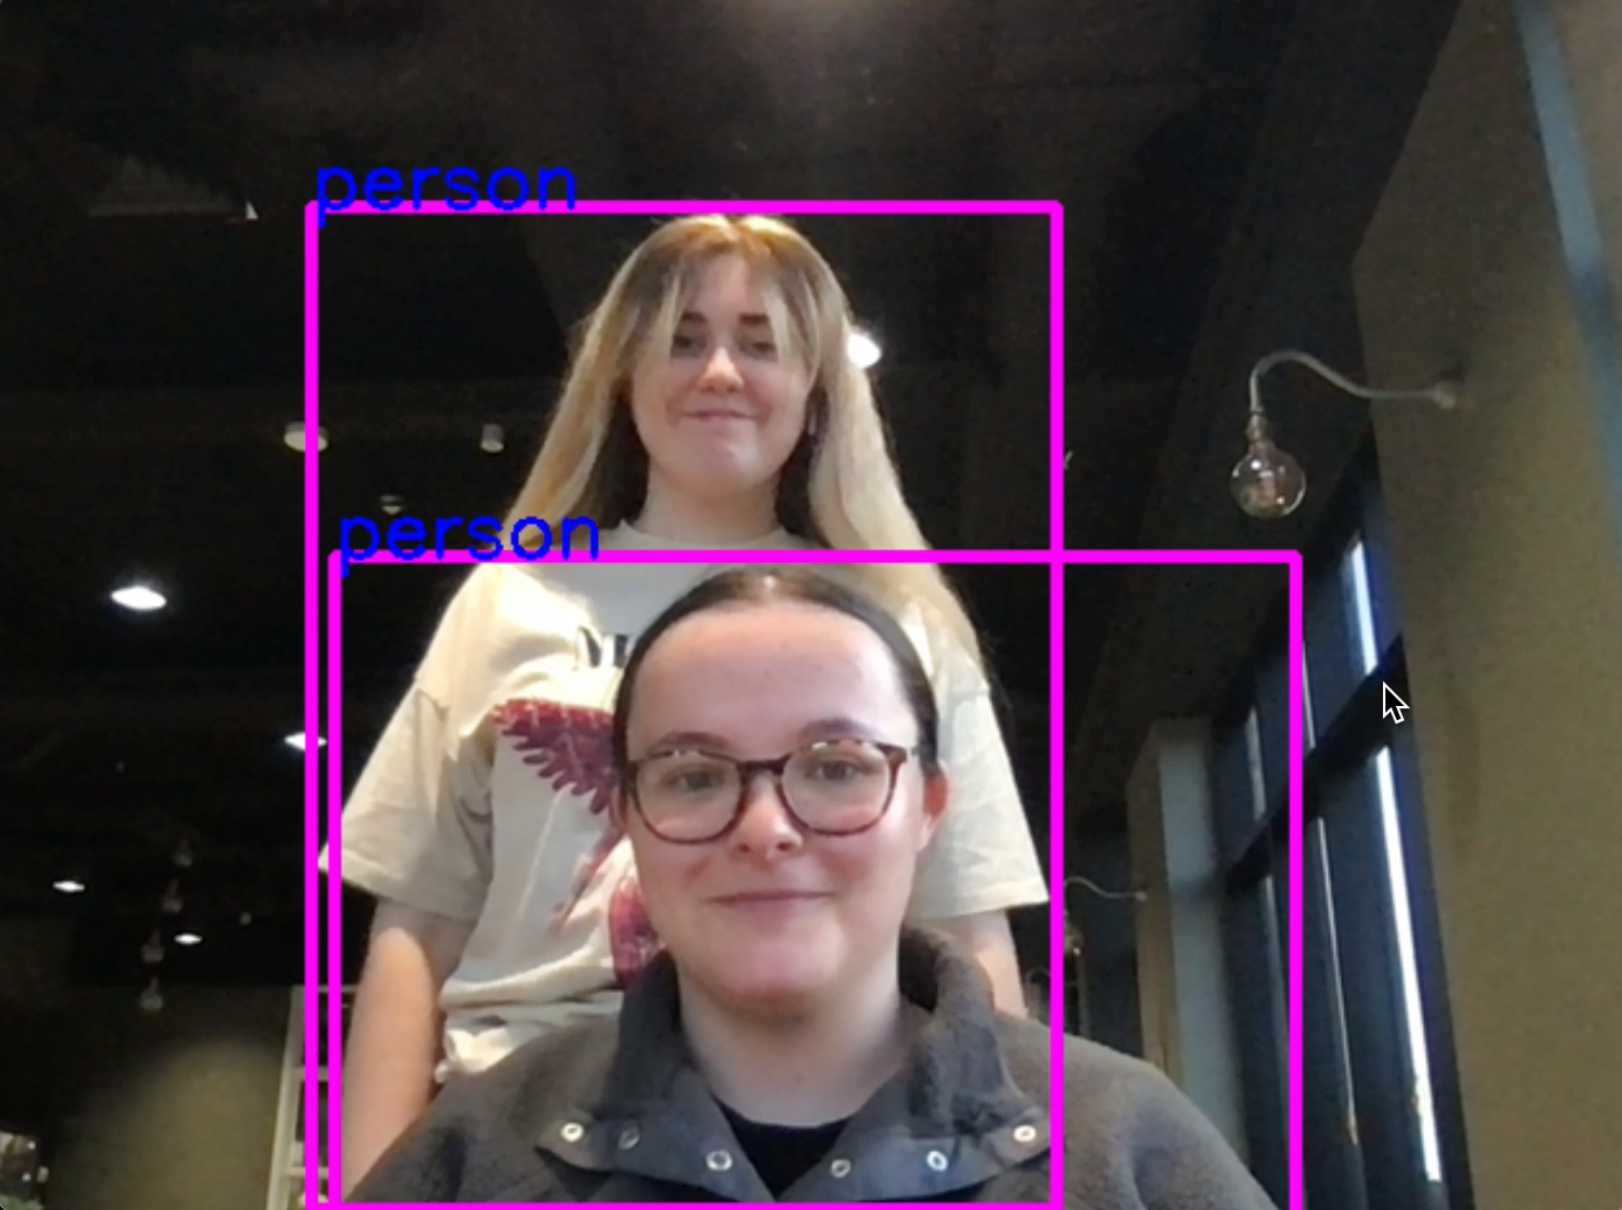
\includegraphics[width=.3\textwidth]{img/fig1-img1.png}\hfill
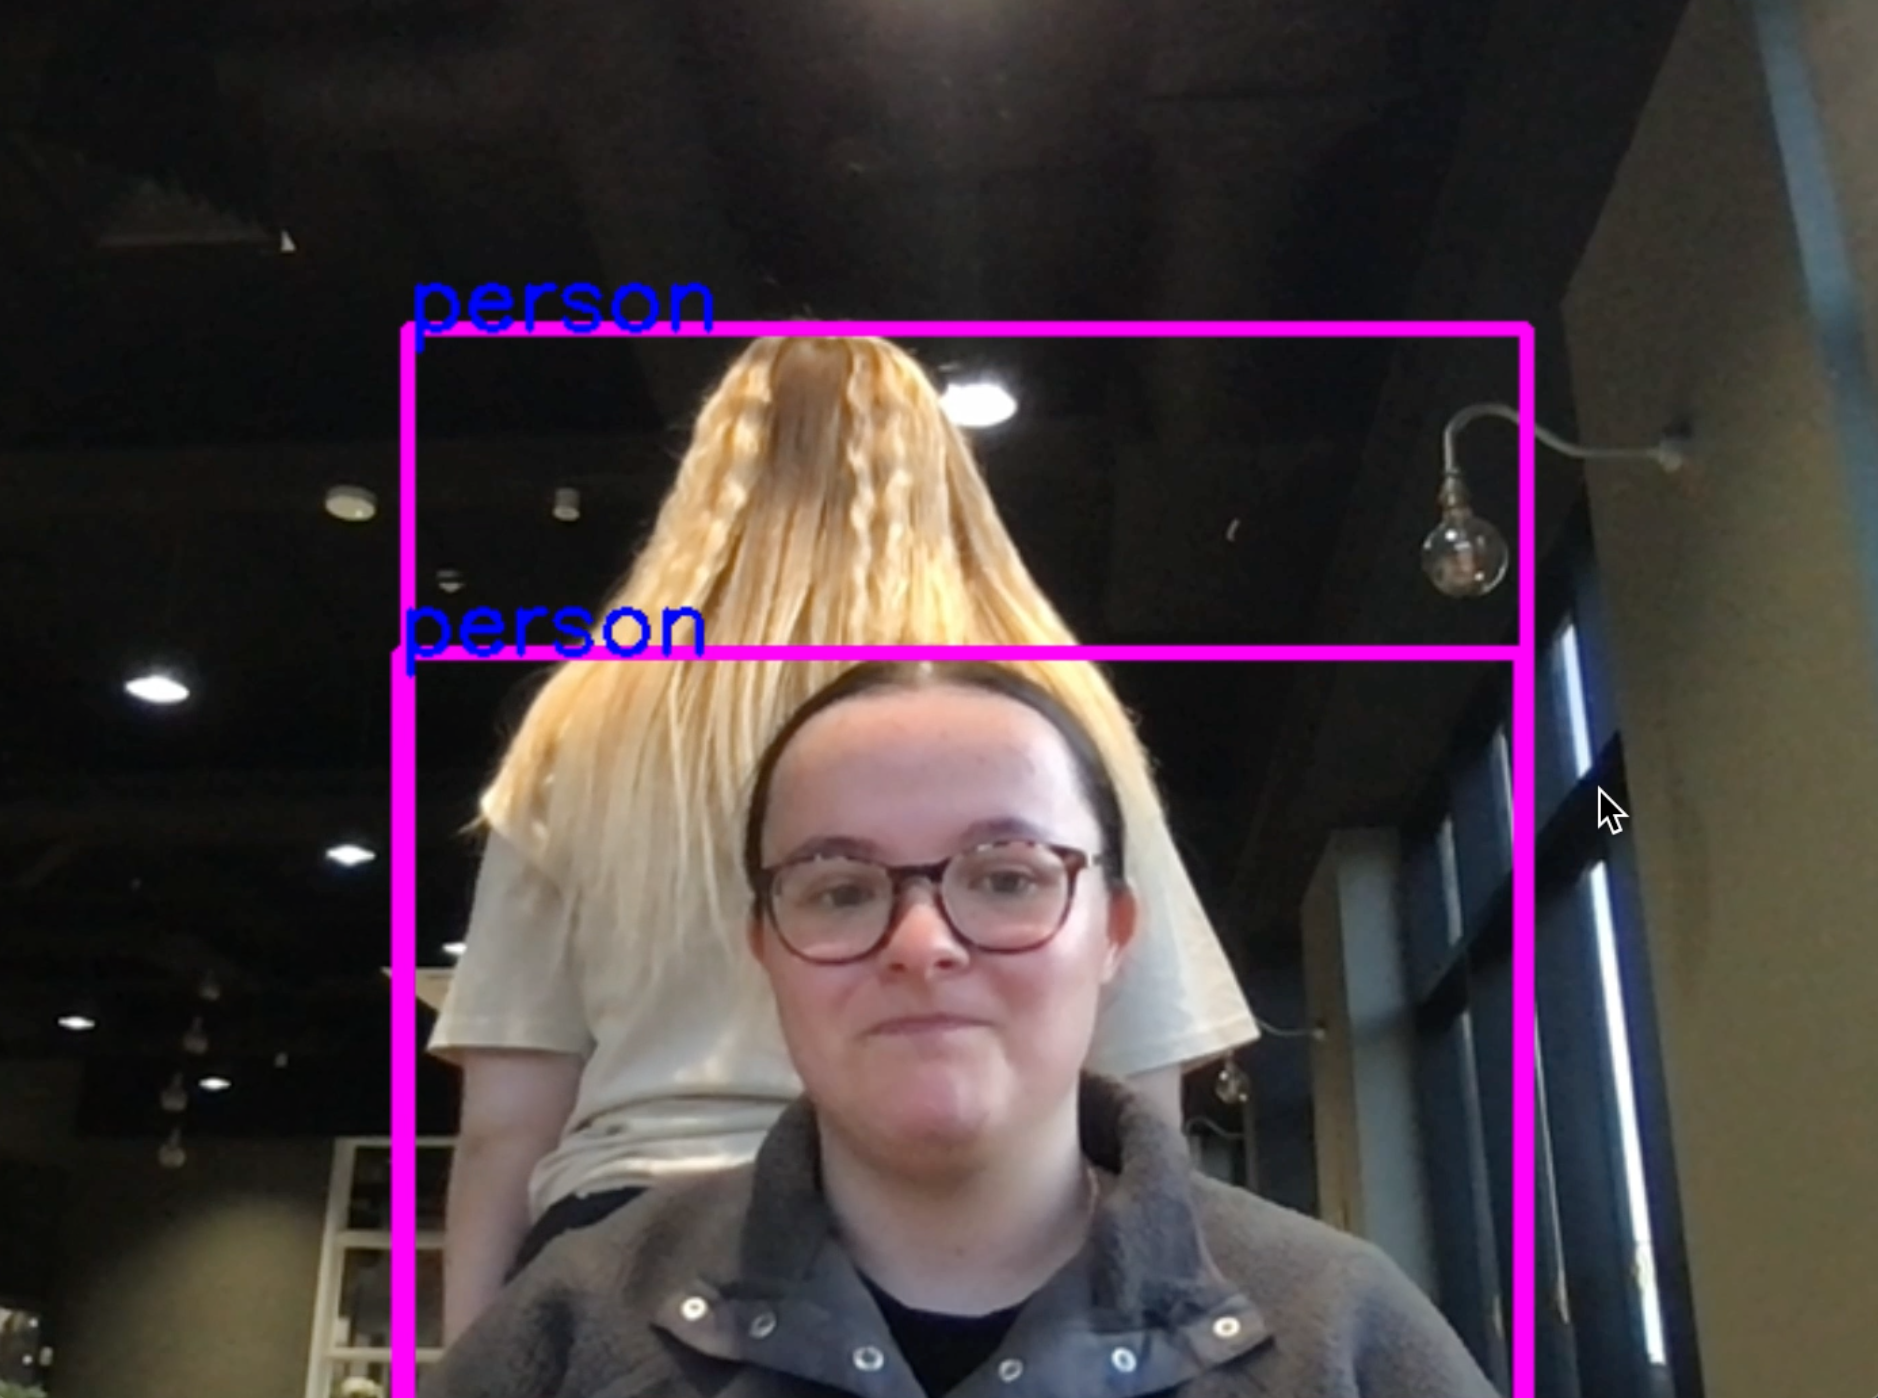
\includegraphics[width=.3\textwidth]{img/fig1-img2.png}\hfill
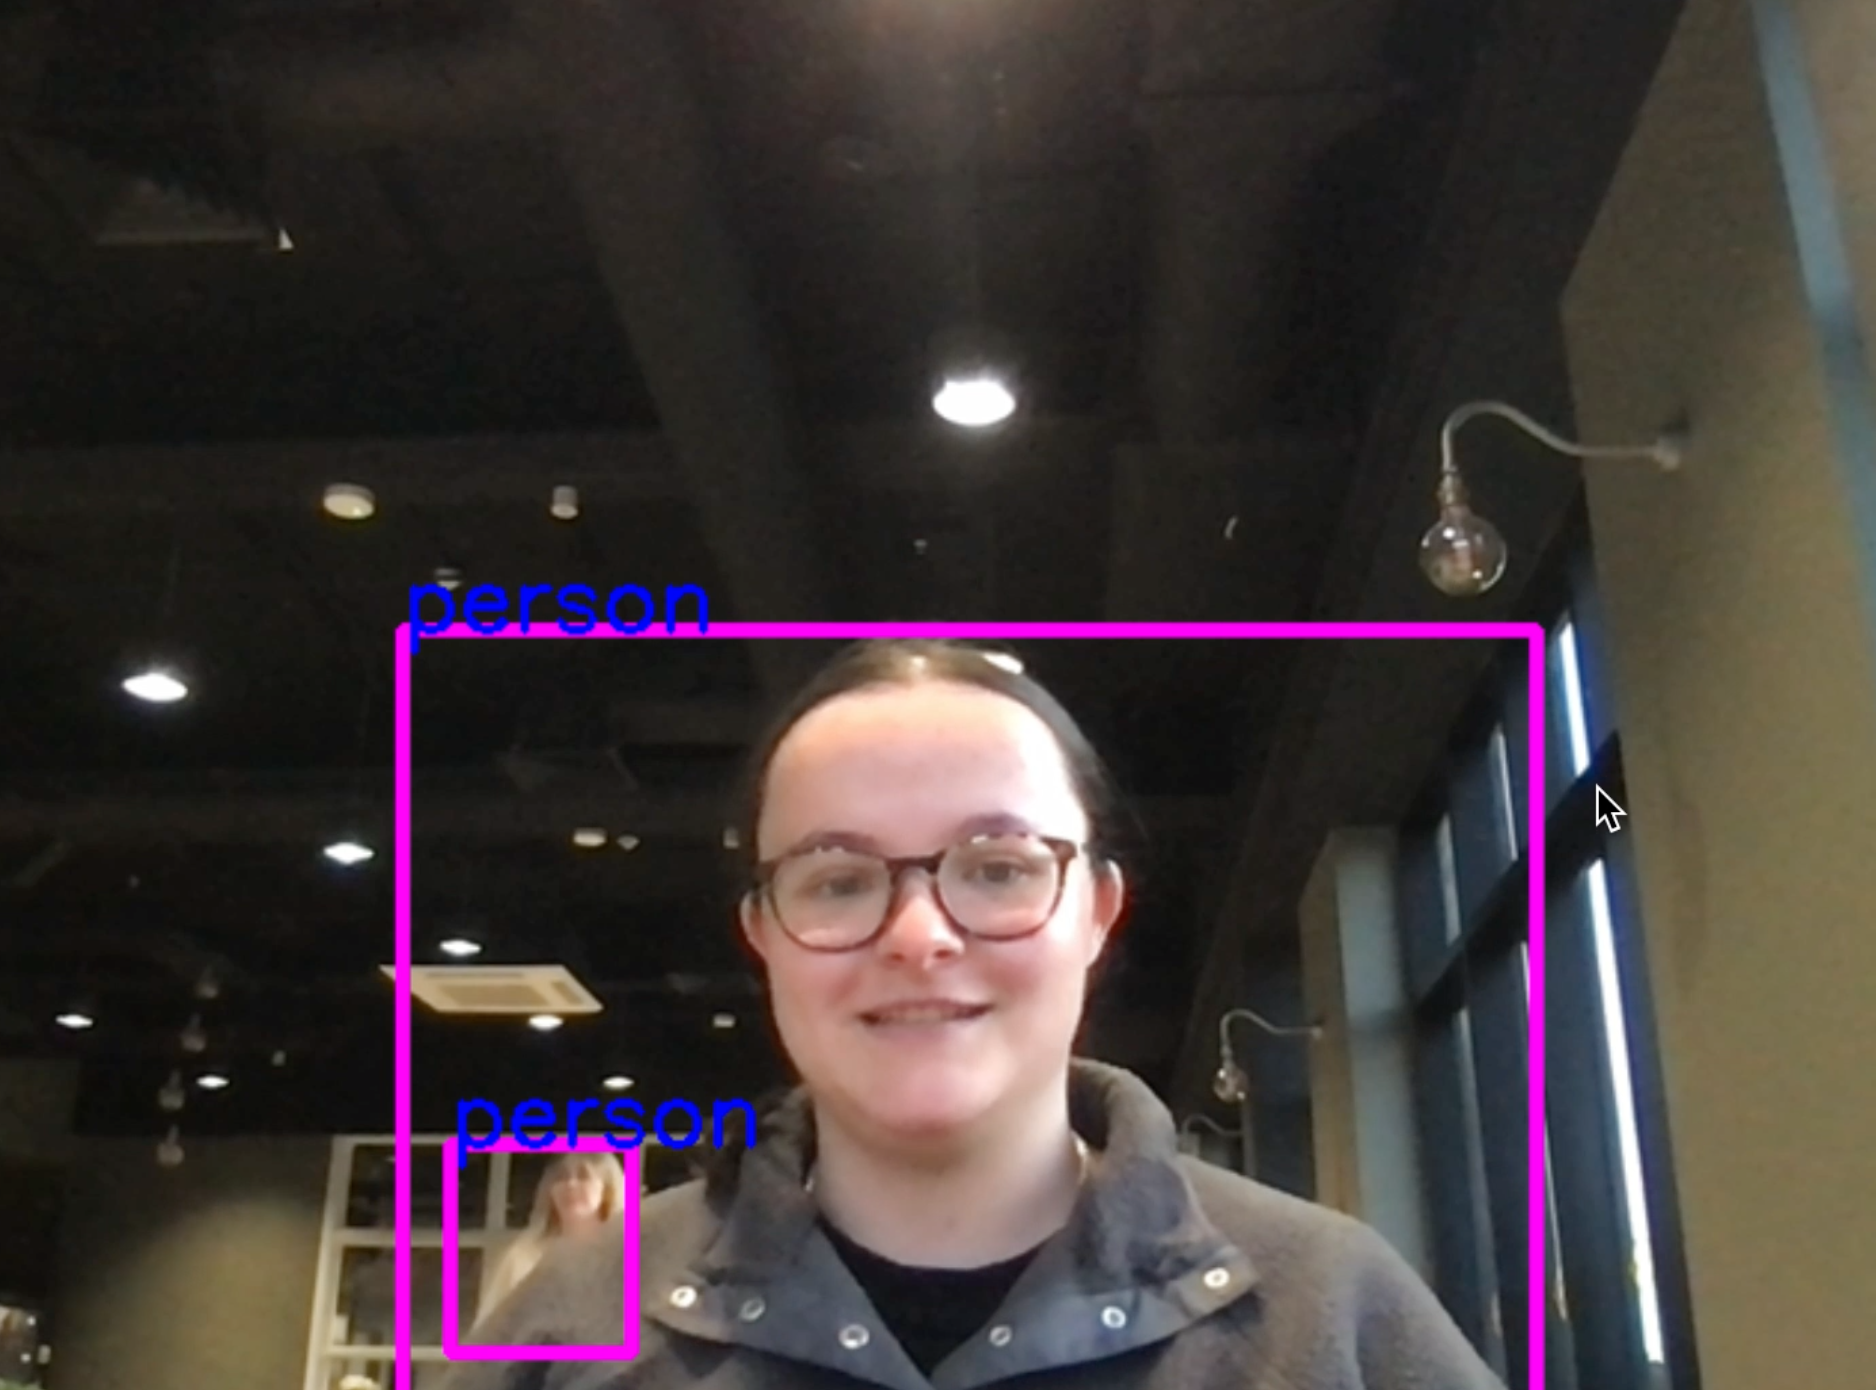
\includegraphics[width=.3\textwidth]{img/fig1-img3.png}\hfill

\caption{YOLO being used to detect more than one person in-front of the camera. The observer stands at different distances and angles to test the system.}
\label{fig:figure1}
\end{figure}

An experiment was carried out to test the limitations that using a front facing camera may have. The user stood 1 meter away from the camera, facing directly in the centre of the screen. They then slowly stepped to the left, decreasing the angle that they were to the screen, ensuring that they maintained a 1-meter distance at all times. As a result, the user was still visible and identifiable by the model until they were at a 35-degree angle to the screen. Figure~\ref{fig:figure2} shows the user where they could first not be identified.
\begin{figure}[ht]
  \centering
  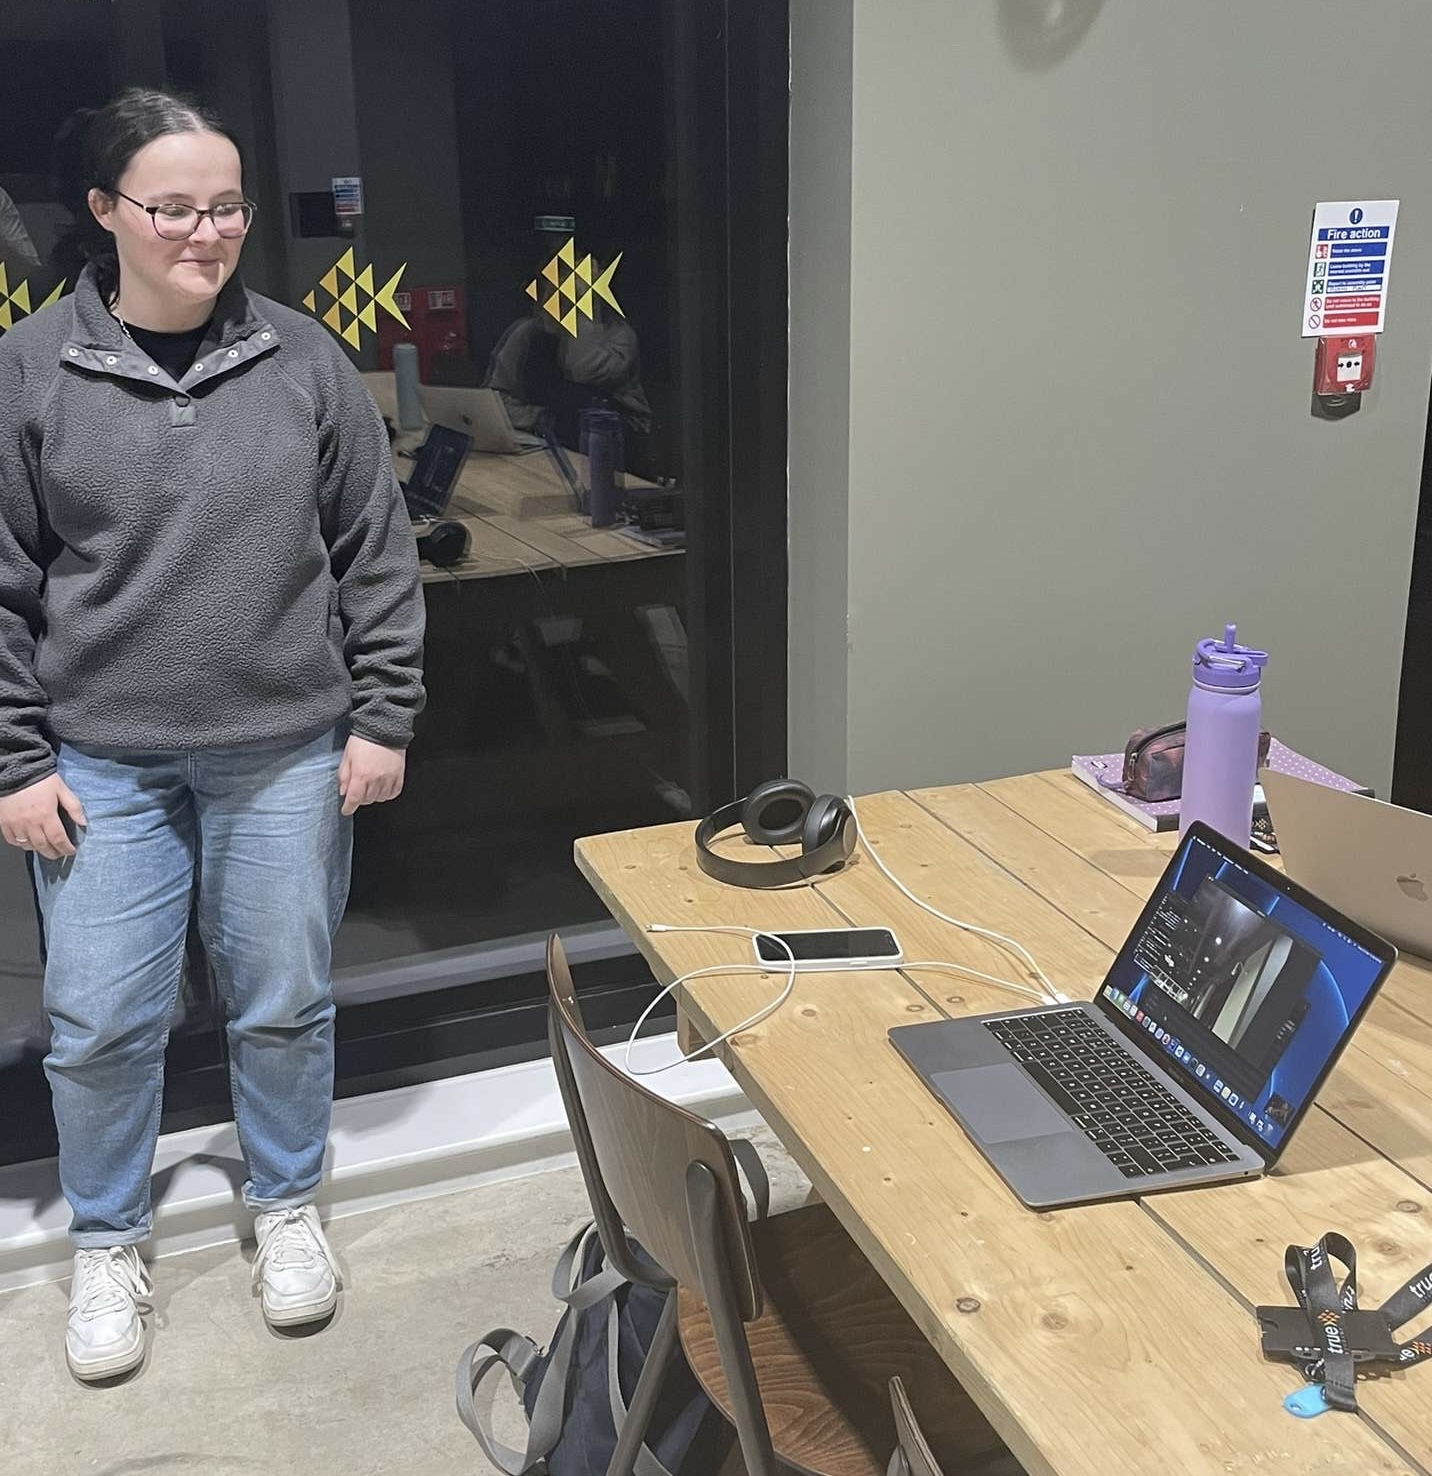
\includegraphics[width=70mm]{img/not_seen.jpg}
  \caption{The angle at which the YOLO model could no longer identify the user. }
  \label{fig:figure2}
\end{figure}

The experiment highlighted the limitations that the YOLO algorithm and camera may have. The user reported that they could still see what was on the screen meaning shoulder surfing could still take place. 
User studies will be carried out during the project to identify if it would be more beneficial to use a fish-eye camera which has a wider-angle view. It will be recorded if the user finds using an external device more cumbersome and if it benefits the results.


It was important to review other detection methods. An eye tracking system was imported from GitHub called GazeTracking (written by Antoine Lame). \textcolor{red}{https://github.com/antoinela me/GazeTracking}.


\textcolor{blue}{The software is free of use, so I have permission to use this. I need to check the permissions of YOLO, but I believe this is the same case.}

\textcolor{blue}{Perhaps I should do some more research about other algorithms and talk about them and justify my choice to compare only these two? }

\textcolor{blue}{The compare the two algorithms, it will be down to the most tests passed. Both have their advantages and disadvantages so there should be discussed.}

\textcolor{purple}{I have written about the two algorithms but this will have to be written academically - most of the content is there though.}

\textcolor{purple}{Background research on Gaza Tracking will have to be done.}

\textcolor{purple}{Permissions will have to be looked into and checked on Uni website.}

\textcolor{purple}{Use an appendix to put test images in? Perhaps just show the important ones in main and then reference appendix. For gaze tracking, I think I should talk about test 2/3 and how it couldn't even identify one person and how they literally had to be directly infront of screen. Then show test 5 and say that there was no chance it would work (but the say about how it detected user 1's eyes.}

\textcolor{purple}{I should maybe suggest that I didn't choose the best eye tracking algorithm? I just say that I didn't know that only one person could be identified at once until I did the testing.}

\textcolor{purple}{Perhaps suggest that the code could be adapted to ignore the direct user (user in this case) and should just look for others - but put in practice, it wouldn't work because at a 1 meter distance +, they can't be tracked (especially when YOLO can track 8+ meters).}

\textcolor{purple}{On that note, talk about how you couldn't test a further distance because the test location room wasn't big enough without moving the screen ('which would then chnage lighting ect. ). However it may not be nessacry as I doubt anyone could read the screen from further than that distence anyway. Maybe suggest that to improve testing, that more than one environemt would be tested and introduce more than one passer-by but back yourself by saying this was to just establish the effectivness of the base algorithm - so these tests should just be done further down the line.}


\subsubsection{Planning tests}
I want to test the following:
\begin{itemize}
    \item The distance at which a person can be identified from.
    \item The number of users that can be identified at once.
    \item The angles to the screen in which the user can still be identified.
\end{itemize}
In order to ensure the tests remain fair, the same devices, environment and users will be used for both. The same tests should be carried out to enable a fair comparison to be made.

Setting the scene -> We will have user1 (the authorised user) and user2 (unauthorised user). A \textcolor{red}{mac camera} will be used for testing purposes but the final product should be tested with various camera hardware. These initial tests should be carried out in the same location in a relatively well lit room. The device should be placed in the same location on a table/flat surface to ensure of a fair test. When distances of the user to the screen are tested, the distance should be precisely tested.

The following 14 tests have been made. 
\begin{enumerate}
    \item User 1 not present. User 2 stands parallel with screen at a \textbf{5 meter distance}. Can User 2 be identified as present?
    \item User 1 not present. User 2 stands parallel with screen at a \textbf{3 meter distance}. Can User 2 be identified as present?
    \item User 1 not present. User 2 stands parallel with screen at a \textbf{2 meter distance}. Can User 2 be identified as present?
    \item User 1 not present. User 2 stands parallel with screen at a \textbf{1 meter distance}. Can User 2 be identified as present?
    \item User 1 sits in-front of screen (to simulate the device being used). User 2 stands \textbf{directly behind} User 1. Can both User 1 and User 2 be detected by the algorithm?
    \item User 1 sits in-front of screen. User 2 stands parallel with screen at a \textbf{5 meter distance}. Can User 1 and User 2 be identified as present?
    \item User 1 sits in-front of screen. User 2 stands parallel with screen at a \textbf{3 meter distance}. Can User 1 and User 2 be identified as present?
    \item User 1 sits in-front of screen. User 2 stands parallel with screen at a \textbf{2 meter distance}. Can User 1 and User 2 be identified as present?
    \item User 1 sits in-front of screen. User 2 stands parallel with screen at a \textbf{1 meter distance}. Can User 1 and User 2 be identified as present?
    \item User 1 sits in-front of screen. Can User 2 be identified from a \textbf{distance further than 5 meters} away from the screen?
    \item User 1 sits in-front of screen. User 2 stands at a 0\degree angle to the screen with a 1-meter distance. Can User 2 be identified?
    \item User 1 sits in-front of screen. User 2 stands at a 45\degree angle to the screen with a 1-meter distance. Can User 2 be identified?
    \item User 1 sits in-front of screen. User 2 stands at a 135\degree angle to the screen with a 1-meter distance. Can User 2 be identified?
    \item User 1 sits in-front of screen. Whilst maintaining a 1-meter distance to the screen, User 2 walks past the device whilst attempting to view what is on screen as much as possible. Can User 2 be identified throughout?
\end{enumerate}

As you can see, tests 1-5 tests distances with just one user. This is important to test \textcolor{blue}{because...}.
Tests 6-10 introduces another user. This is to replicate the idea of there being one person using the device with another attempting to shoulder surf.
Tests 11-13 checks the ability of the camera and algorithm to identify users stood at various angles to the camera.
The purpose of test 14 is to simulate a user attempting to view what is on screen whilst passing by. Whilst this may not be done maliciously, it is important the algorithm can track people walking past so that it can be developed further to detect shoulder surfing.

A successful test suite would mean that all the tests pass except from test 11 when using the \textcolor{red}{mac camera with spec x,y, z}. \textcolor{blue}{Test 11 should fail because it's a front facing camera}.

\textcolor{red}{Check tenses here please.}

\subsubsection{Carrying out tests}

Set up in a room with good lighting. MacBook was used and stayed in the same location throughout. A tape measure was used to check the distances. The same two users were used throughout.

Put some images here. 

\subsubsection{Evaluating tests}

So, after testing, we know that the person detection is a lot better. One issue I found is that it was quite laggy, as there's so much computation. We have a constant accuracy percentage being outputted – perhaps reduce this. It’s also trying to detect other things other than people; can we get rid of this. This would definitely speed up the algorithm.

Unfortunately I didn't do all of the tests for the GazeTracking algorithm. Was this a good idea? For the next testing stage, I want to ensure I produce more tests. No point doing tests 6-14 as two users were used but the algorithm could identify only one. I did check if the use of glasses was effecting it, but they weren't.

\subsubsection{Creating the initial prototype}
Write about the code you made for the inital prototype. this was basic python code that used YOLO to detect people. it currently identifies a shoulder surfer if there is more than one person detected (suggesting the second person is the shoulder surfer) however this is not accurate and should be changed for the final product. A basic UI was created so that the detector can be turned on/off. The camera livestream is used whenever the code is running - it doesn't stop accessing the camera even if the stop button is pressed. An alert noise was found online (check the permissions for this). I struggled to create the brightness decrease - talk about how you first just made a 'blur' but this did not work properly on macOS so you chnaged it to access mac shortcuts (i think that's what it is). talk about how it isnt yet usable for all OS's - currently only mac so this needs to be changed. make sure you put some code snippits in here to look cool.

% Long form code listings can be taken directly from an external file.
\lstinputlisting[language={python}, firstline=38, lastline=72 label={lst:useryolo}, caption={An
  implementation of some amazing code.}]{./listings/useryolo.py}

\subsubsection{Initial prototype User study}
planning
execution
results

% Prints the Reference section
\printbibliography

% Appendices are used to provide bulk information that does not fit
% into the main text. Common content is program code and data
% sets. You may want to discuss key elements in the main text, but
% provide the rest in an appendix for completeness.
\clearpage\appendix

\end{document}
